% =====================================================================
%  Reporte.tex
%  ========================
%
%
%  Descripción:
%  ------------
%  Reporte de la tarea de correlación y regresión de Matemáticas para
%  la Computación: un modelo lineal para el precio de los anuncios de
%  Airbnb en la Ciudad de México, con el corte de septiembre de 2026.
%  Usa la clase LNCS de Springer, pero sin bloque de título y en tono
%  coloquial.
%
%
%  Considerations:
%  ------------
%  - Compila con pdflatex y latexmk; llncs.cls viene en TeX Live
%  - Todas las cifras salen de Regresion.ipynb, y las figuras de
%    figuras/ las escribe el mismo notebook
%
%
%  Metadata:
%  ----------
%   * Author : zxxz6 (Bryan Violante Arriaga)
%   * Version: 1.1.3
%
%
%  History:
%  ------------
%  Author      Date            Description
%  zxxz6       13/11/2026      Las variables del texto coinciden con el
%                              modelo; ortografia y redaccion
%  zxxz6       12/11/2026      Margenes de 2.5 cm; la matriz de correlacion
%                              cabe en la primera hoja
%  zxxz6       12/11/2026      Titulo Actividad en lugar del nombre de la
%                              tarea
%  zxxz6       12/11/2026      Mas corto y coloquial, sin bloque de titulo
%  zxxz6       12/11/2026      Creation
%
%
% =====================================================================
\documentclass{llncs}

\usepackage[letterpaper,margin=2.5cm]{geometry}
\usepackage[T1]{fontenc}
\usepackage[spanish,es-noshorthands,es-tabla,es-nodecimaldot]{babel}
\usepackage{graphicx}
\usepackage{booktabs}
\usepackage{amsmath}
\usepackage{array}
\usepackage[hidelinks]{hyperref}
\urlstyle{same}

\graphicspath{{figuras/}}

\renewcommand{\topfraction}{0.85}
\renewcommand{\textfraction}{0.1}
\renewcommand{\floatpagefraction}{0.8}

\newcolumntype{L}[1]{>{\raggedright\arraybackslash}p{#1}}

\begin{document}

\renewcommand{\figurename}{Fig.}
\renewcommand{\tablename}{Tabla}
\pagestyle{plain}

\noindent Bryan Violante Arriaga \hfill Matemáticas para la
Computación\\
\phantom{x}\hfill 13 de noviembre de 2026
\medskip\hrule\bigskip

\bigskip

{\centering\Large\bfseries Actividad\par}

\bigskip


Para esta tarea se usaron los datos de Airbnb de la Ciudad de México, el mismo
dataset del proyecto, el corte de septiembre de 2026 de Inside
Airbnb\footnote{\url{https://insideairbnb.com/get-the-data/}}. La idea principal
es ver de qué depende el precio por noche de un anuncio (en el proyecto se
detalla más). Para esta actividad se conservan
los 24,763 anuncios que tienen precio entre 100 y 50 mil pesos y
calificación.

Es importante aclarar que el modelo desarrollado es explicativo y no
predictivo, o sea que no buscamos predecir el precio sino entender cómo
cambia.

\bigskip

\textbf{Disclaimer:} Esta actividad se realizó con ayuda de herramientas de
IA para el análisis de los datos y la generación de gráficos, así como para
la generación del código de la actividad.


\section*{Selección de las variables}

Se partió con once variables numéricas que podían tener que ver con el
precio: capacidad, recámaras, camas, baños, distancia al Ángel de la
Independencia, calificación, número de reseñas, días disponibles al
año, noches mínimas, cuántos anuncios tiene el anfitrión y cuántos
años lleva en Airbnb. Posteriormente se obtuvo la correlación de
Spearman entre todas las variables. Se usó Spearman porque varias tienen
valores muy extremos, como anfitriones con cientos de anuncios, y Pearson
tiende a dejarse llevar por esos valores.

\begin{figure}[h!]
\centering
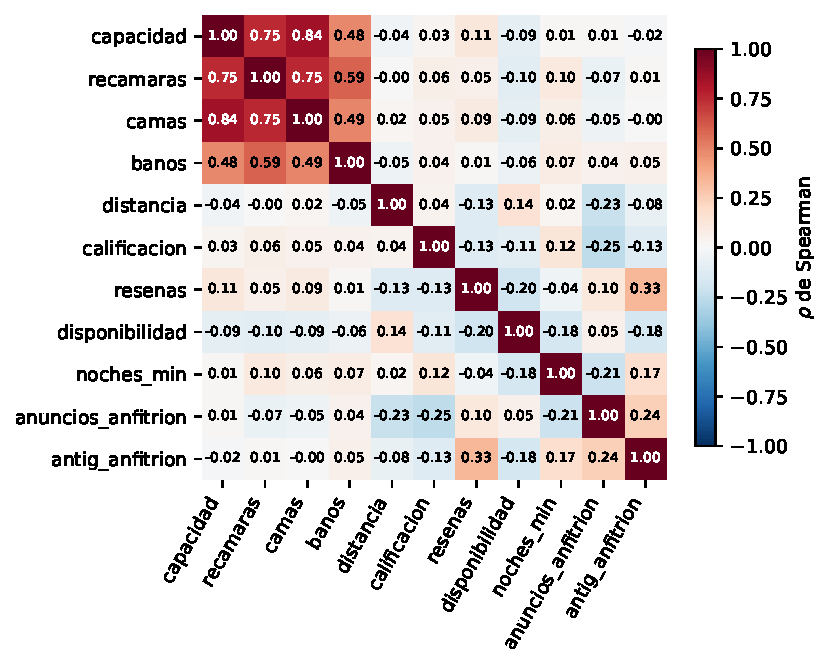
\includegraphics[width=0.76\textwidth]{Correlacion.pdf}
\caption{Matriz de correlación de Spearman entre las once variables.}
\label{fig:correlacion}
\end{figure}

\newpage

Capacidad, recámaras y camas son casi la misma
cosa: la correlación entre ellas va de 0.75 a 0.84, y los baños andan
cerca, alrededor de 0.5. Todas miden qué tan grande es el lugar, así que
solo una de ellas puede entrar al modelo.

Para escoger se probaron todas las combinaciones de tres variables, se
conservaron las que no tenían ningún par con correlación arriba de 0.3,
y de esas se seleccionó la que más se relacionaba con el precio:
\textbf{capacidad, distancia y calificación}. La correlación más alta
entre ellas es de 0.04, y cada una mide algo completamente distinto
(tamaño, ubicación y calidad).


\section*{Cómo se ven}

\begin{figure}
\centering
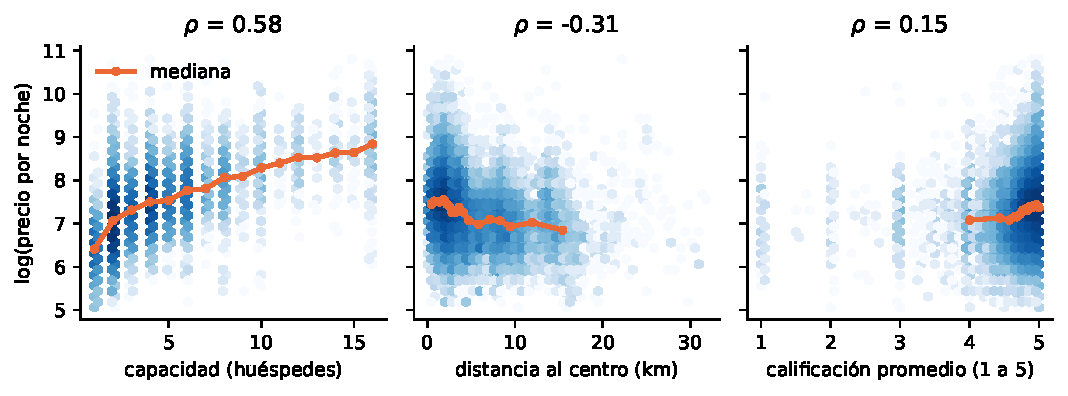
\includegraphics[width=\textwidth]{Dispersion.pdf}
\caption{El logaritmo del precio contra cada variable. Entre más
oscuro el hexágono, más anuncios; la línea naranja es la mediana.}
\label{fig:dispersion}
\end{figure}

En la Fig.~\ref{fig:dispersion} se puede ver cómo el precio sube con la
capacidad, pero cada huésped extra suma menos que el anterior. Con la
distancia el precio baja rápido en los primeros 3\,km y luego casi se
aplana. La calificación es la más débil, porque casi todos tienen entre
4.5 y 5, y muchos de los que tienen 5 perfecto son anuncios nuevos con
pocas reseñas (la mediana es de 4).


\section*{El modelo}

Primero se ajustó el precio contra las tres variables tal cual. Salió un
$R^2$ de 0.26, pero con residuos muy sesgados: unos cuantos anuncios
carísimos movían todo el ajuste, y entre más caro el anuncio, más grande
el error.

Después se tomó el logaritmo del precio para aplanar los precios altos,
y el $R^2$ subió a 0.38. Los residuos todavía mostraban que el modelo se
pasaba con los lugares muy chicos y muy grandes, y algo parecido con la
distancia, así que también se tomó el logaritmo de la capacidad y de la
distancia. El modelo final, con $R^2 = 0.425$, es
\begin{align*}
\log(\text{precio}) = 5.959 &+ 0.717\,\log(\text{capacidad}) \\
&- 0.182\,\log(\text{distancia}) + 0.164\,\text{calificación}
\end{align*}


\begin{table}
\caption{Coeficientes del modelo final, con su error estándar entre
paréntesis.}
\label{tab:betas}
\centering
\begin{tabular}{@{}lcL{8.5cm}@{}}
\toprule
Variable & $\hat\beta$ & Qué quiere decir \\
\midrule
log(capacidad) & 0.717 (0.013) & De 2 a 4 huéspedes, el precio sube
64\,\% \\
log(distancia) & $-0.182$ (0.009) & De 2 a 8\,km del Ángel, el precio
baja 22\,\% \\
calificación & 0.164 (0.020) & De 4.5 a 5 estrellas, el precio sube
8.5\,\% \\
intercepto & 5.959 (0.101) & Nada útil: sería un lugar con cero
estrellas \\
\bottomrule
\end{tabular}
\end{table}

Los tres coeficientes son distintos de cero. Los errores estándar se
calcularon agrupando por anfitrión, porque un mismo anfitrión sube
muchos anuncios parecidos y no son independientes. Si no se hacía así,
los errores salían como de la mitad y el modelo parecía más preciso de
lo que es.


\section*{Resultados}

\begin{figure}
\centering
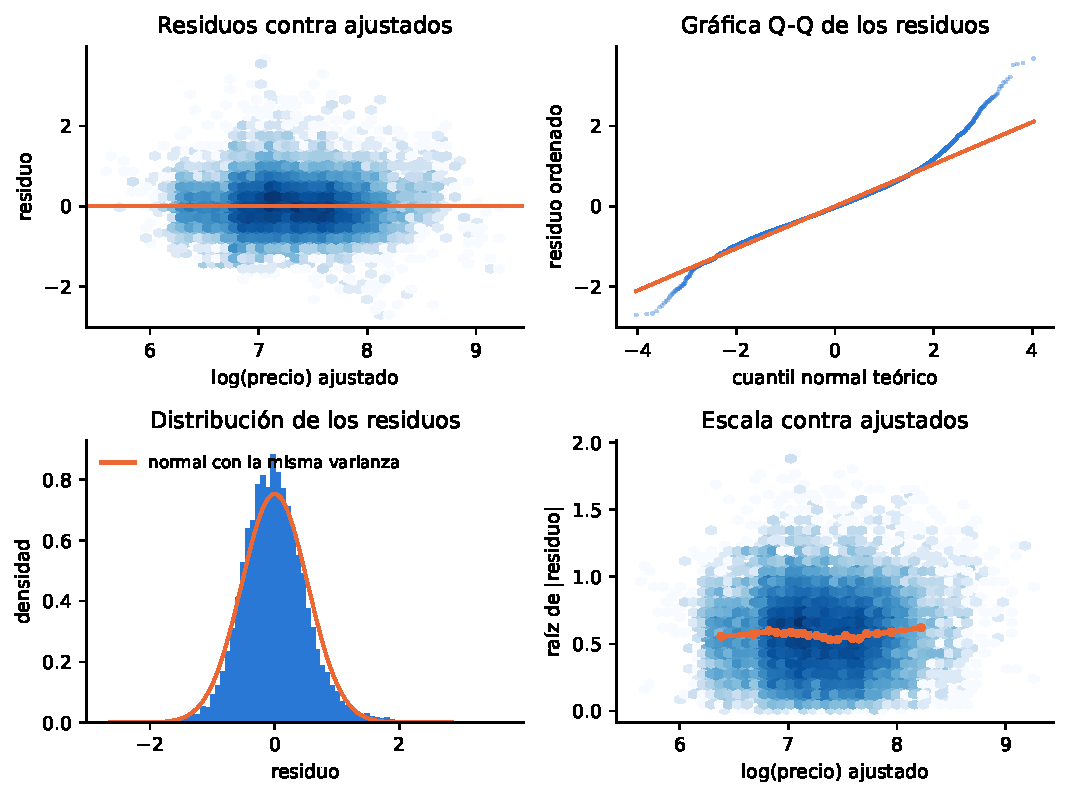
\includegraphics[width=0.75\textwidth]{Diagnostico.pdf}
\caption{Los residuos del modelo final.}
\label{fig:diagnostico}
\end{figure}

En la Fig.~\ref{fig:diagnostico} los residuos quedan centrados en cero
y sin ninguna forma rara. La gráfica Q-Q es casi una recta (solo se
despega arriba), porque hay más anuncios caros de los que esperaría
una normal. La dispersión de los errores es casi pareja.

Para comprobar que no fuera suerte, se separó el 20\,\% de los
anuncios, se ajustó el modelo con el resto y se probó en esos: el $R^2$
salió igual, 0.425. Eso sí, para predecir no es gran cosa: en la mediana
se equivoca por 434 pesos, como un tercio del precio. Es normal, porque
le faltan cosas importantes.

Lo que el modelo no logra arreglar es la distancia: dos colonias a la
misma distancia del Ángel pueden tener precios muy distintos, y eso ya
no se corrige con logaritmos.

\section*{Conclusiones}

Con tres variables y unos logaritmos se explica aproximadamente el
43\,\% de la variación del precio. Lo que falta es dónde está
exactamente el lugar y qué tipo de lugar es.

\section*{Limitaciones}

\begin{itemize}
\item No es causa y efecto. Agrandar la vivienda no garantiza cobrar
64\,\% más.
\end{itemize}




\end{document}

%############################# END OF REPORTE.TEX ##############################
%###############################################################################
